\chapter{Substâncias puras e misturas}\label{ch:g6:pure-substances-and-mixtures}

O rótulo de uma garrafa de água mineral lista uma dúzia de substâncias
dissolvidas, com as quantidades em miligramas por litro. A água que sai
do purificador de um laboratório não lista nenhuma. As duas são límpidas
e incolores, as duas matam a sede --- e, no entanto, só uma delas é o
que um químico chama de pura. Este capítulo dá à palavra ``pura'' o seu
sentido exato, e mostra como distinguir uma \omterm{def:g6:pure-substances-and-mixtures:pure-substance}{substância pura} de uma
\omterm{def:g6:pure-substances-and-mixtures:mixture}{mistura} sem provar nada.

\begin{recall}
\omterm{def:g2:mixing-and-dissolving:mix}{Misturar} é juntar coisas diferentes; um sólido que \omterm{def:g2:mixing-and-dissolving:dissolve}{se dissolve} na água
deixa o líquido límpido, e o líquido límpido é uma solução
(\cref{ch:g2:mixing-and-dissolving}). As \omterm{def:g6:pure-substances-and-mixtures:mixture}{misturas} podem ser separadas
por \omterm{def:g3:separating-mixtures:sieve}{peneiração}, \omterm{def:g3:separating-mixtures:decant}{decantação}, \omterm{def:g3:separating-mixtures:filter}{filtração} e \omterm{def:g3:separating-mixtures:evaporate}{evaporação}
(\cref{ch:g3:separating-mixtures}). Todo material tem propriedades que
podem ser testadas: duro ou macio, transparente ou não, flutua ou afunda
(\cref{ch:g1:materials-around-us}).
\end{recall}

\section{Espécies químicas e substâncias puras}

\begin{definition}[Espécie química]\label{def:g6:pure-substances-and-mixtures:species}
Uma \emph{espécie química}\index{especie quimica@espécie química} é um tipo determinado
de substância, com nome próprio e propriedades próprias: a água, o
açúcar, o sal, o oxigênio, o etanol (o álcool do vinho), o ferro.
\end{definition}

\begin{definition}[Substância pura]\label{def:g6:pure-substances-and-mixtures:pure-substance}
Uma \emph{substância pura}\index{substancia pura@substância pura} é formada por uma única
\omterm{def:g6:pure-substances-and-mixtures:species}{espécie química} e mais nada: a água destilada, um cristal de açúcar, um
anel de ouro puro.
\end{definition}

\begin{definition}[Mistura]\label{def:g6:pure-substances-and-mixtures:mixture}
Uma \emph{mistura}\index{mistura} contém várias \omterm{def:g6:pure-substances-and-mixtures:species}{espécies químicas}. O \omterm{def:g4:air-a-mixture-of-gases:air}{ar},
a água do mar, a água mineral, o leite, o granito e o suco de laranja
são misturas.
\end{definition}

\begin{remark}[Puro na linguagem do dia a dia]\label{rem:g6:pure-substances-and-mixtures:everyday}
Uma caixa de ``suco de laranja puro'' quer dizer que nada foi
acrescentado ao suco. Para um químico, o suco continua sendo uma
\omterm{def:g6:pure-substances-and-mixtures:mixture}{mistura}: água, açúcares, ácidos, vitaminas, corantes e aromas, muitas
\omterm{def:g6:pure-substances-and-mixtures:species}{espécies químicas}. A ``água pura da montanha'' também é uma \omterm{def:g6:pure-substances-and-mixtures:mixture}{mistura}:
água com sais dissolvidos.
\end{remark}

\begin{omfigure}
\begin{tikzpicture}[font=\small, level distance=1.55cm,
    box/.style={draw=omDef, fill=omDef!6, rounded corners=2pt, align=center,
      inner sep=4pt},
    level 1/.style={sibling distance=7.2cm},
    level 2/.style={sibling distance=3.6cm},
    edge from parent/.style={draw, thick, omDef, ->}]
  \node[box] {matéria}
    child {node[box] {substância pura\\ \footnotesize uma espécie química}
      child {node[box, draw=black!40, fill=white] {água destilada,\\ sal, ferro}}}
    child {node[box] {mistura\\ \footnotesize várias espécies químicas}
      child {node[box] {homogênea\\ \footnotesize um só aspecto}
        child {node[box, draw=black!40, fill=white] {água salgada,\\ ar}}}
      child {node[box] {heterogênea\\ \footnotesize partes visíveis}
        child {node[box, draw=black!40, fill=white] {água barrenta,\\ granito}}}};
\end{tikzpicture}

{\small A classificação da matéria. As caixas de baixo dão exemplos de
cada tipo.}
\end{omfigure}

\section{Misturas homogêneas e heterogêneas}

\begin{definition}[Misturas homogêneas e heterogêneas]\label{def:g6:pure-substances-and-mixtures:homogeneous}
Uma \omterm{def:g6:pure-substances-and-mixtures:mixture}{mistura} é uma \emph{mistura homogênea}\index{mistura homogenea@mistura homogênea}
quando suas diferentes partes não podem ser distinguidas a olho nu, nem
mesmo com uma lupa: ela tem o mesmo aspecto em toda parte. Ela é uma
\emph{mistura heterogênea}\index{mistura heterogenea@mistura heterogênea} quando pelo menos
duas partes diferentes podem ser vistas.
\end{definition}

\begin{example}[Quatro misturas]\label{ex:g6:pure-substances-and-mixtures:four}
A água salgada e o \omterm{def:g4:air-a-mixture-of-gases:air}{ar} são homogêneos: suas partes não podem ser vistas.
O óleo sobre a água é heterogêneo: duas camadas. A água barrenta é
heterogênea: grãos ficam em suspensão nela e se depositam. O suco de
laranja com polpa é heterogêneo: os pedacinhos de polpa podem ser vistos.
\end{example}

\begin{omfigure}
\begin{tikzpicture}[font=\small, scale=1.15]
  \pic[transform shape] at (0,0) {beaker={0.7}{omWater!80}};
  \node[anchor=north, align=center] at (0,-0.15) {água salgada:\\ homogênea};
  \pic[transform shape] at (2.6,0) {beaker={0.7}{omWater!80}};
  \fill[yellow!55!orange!60] (1.8,1.05) rectangle (3.4,1.4);
  \draw[omGlass, line width=0.7pt] (1.8,1.05) -- (1.8,1.4) (3.4,1.05) -- (3.4,1.4);
  \node[anchor=north, align=center] at (2.6,-0.15) {óleo sobre água:\\ heterogênea};
  \pic[transform shape] at (5.2,0) {beaker={0.7}{brown!25}};
  \foreach \x/\y in {4.6/0.3,4.9/0.7,5.3/0.5,5.6/1.0,5.0/1.1,5.4/0.2,5.8/0.6}
    \fill[brown!65] (\x,\y) circle (0.04);
  \fill[brown!60] (4.4,0) rectangle (6.0,0.12);
  \node[anchor=north, align=center] at (5.2,-0.15) {água barrenta:\\ heterogênea};
  \pic[transform shape] at (7.8,0) {beaker={0.7}{orange!45}};
  \foreach \x/\y in {7.3/0.35,7.6/0.8,8.0/0.5,8.3/1.0,7.7/1.15,8.2/0.25,7.45/0.65}
    \fill[orange!80!brown] (\x,\y) ellipse (0.08 and 0.03);
  \node[anchor=north, align=center] at (7.8,-0.15) {suco com polpa:\\ heterogênea};
\end{tikzpicture}

{\small Uma \omterm{def:g6:pure-substances-and-mixtures:homogeneous}{mistura homogênea} e três \omterm{def:g6:pure-substances-and-mixtures:homogeneous}{misturas heterogêneas}.}
\end{omfigure}

\begin{omfigure}
\begin{minipage}[b]{0.48\linewidth}\centering
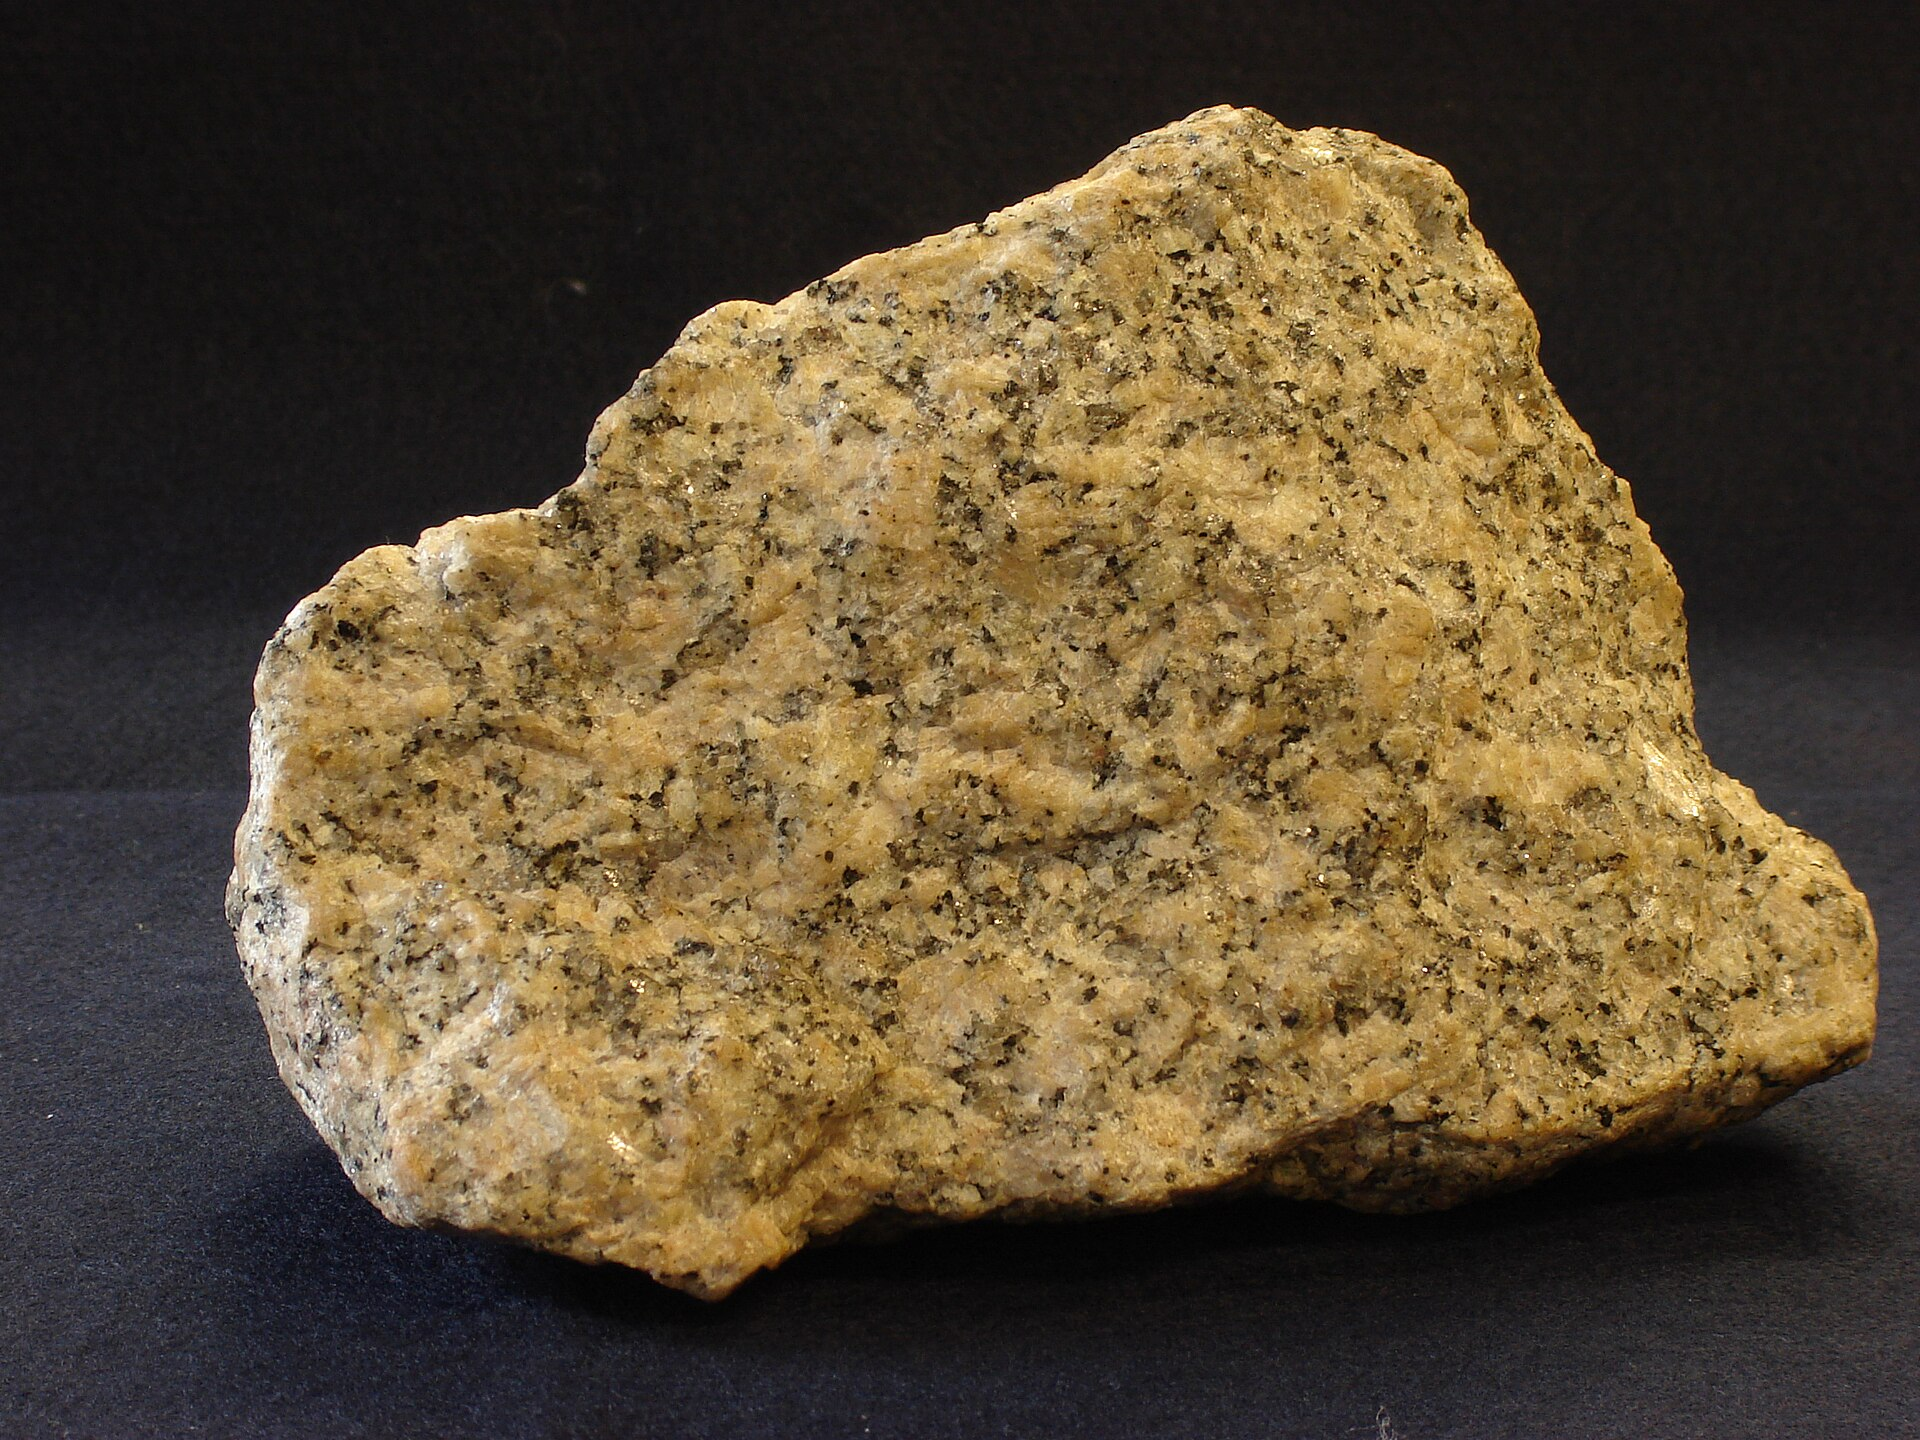
\includegraphics[width=\linewidth,height=4.6cm,keepaspectratio]{images/book1/granite.jpg}

{\small O granito: dá para ver grãos de três ou quatro minerais
diferentes. Um sólido heterogêneo. Foto: Eurico Zimbres, CC BY-SA 2.0 br.}
\end{minipage}\hfill
\begin{minipage}[b]{0.48\linewidth}\centering
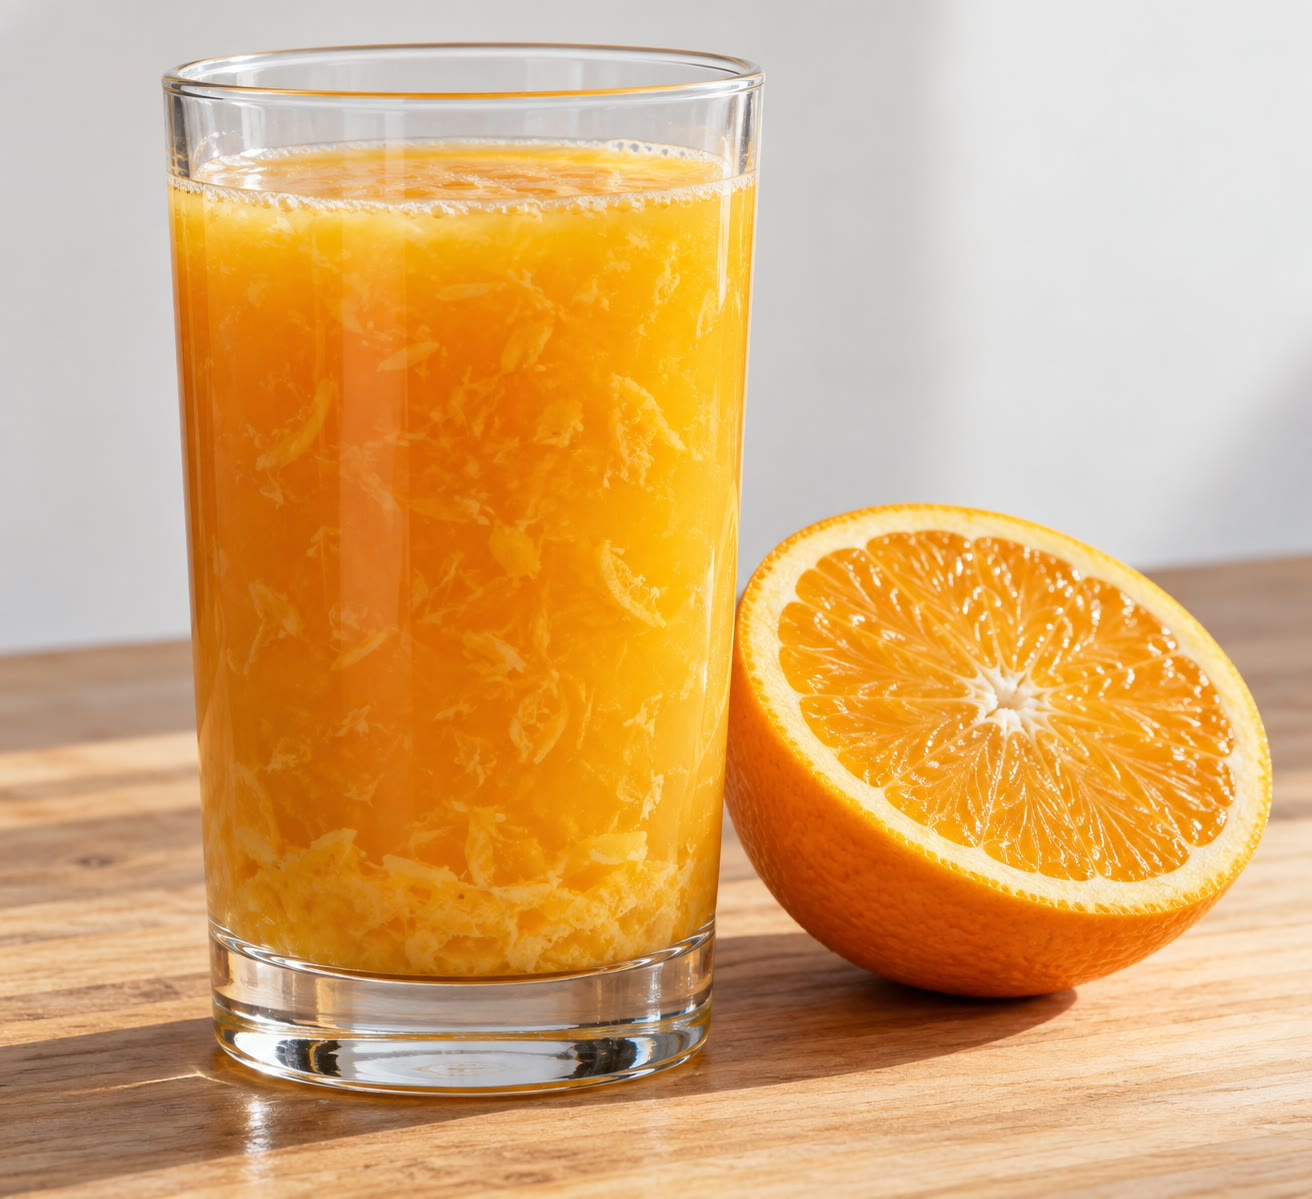
\includegraphics[width=\linewidth,height=4.6cm,keepaspectratio]{images/book1/ai/g6-orange-juice.jpg}

{\small Suco de laranja com polpa: uma \omterm{def:g6:pure-substances-and-mixtures:homogeneous}{mistura heterogênea}.}
\end{minipage}
\end{omfigure}

\begin{remark}[Homogêneo não quer dizer puro]\label{rem:g6:pure-substances-and-mixtures:not-pure}
A água salgada tem exatamente o aspecto da água pura. Olhar não basta
para distinguir uma \omterm{def:g6:pure-substances-and-mixtures:pure-substance}{substância pura} de uma \omterm{def:g6:pure-substances-and-mixtures:homogeneous}{mistura homogênea}: é preciso
medir alguma coisa.
\end{remark}

\section{Identificar uma substância pura por suas constantes}

\begin{proposition}[Uma substância pura tem constantes próprias]\label{prop:g6:pure-substances-and-mixtures:constants}
% ledger: mp:water, bp:water, bp:ethanol, mp:ethanol, rho:water, rho:ethanol, mp:NaCl, mp:Fe, rho:Fe
Cada \omterm{def:g6:pure-substances-and-mixtures:pure-substance}{substância pura} funde a uma temperatura fixa própria, ferve a uma
temperatura fixa própria (à pressão normal) e tem uma massa própria para
um dado volume, a sua densidade. Esses números são as suas constantes; o
livro de física explica o que elas medem. Para algumas \omterm{def:g6:pure-substances-and-mixtures:pure-substance}{substâncias puras}:
\begin{center}
\small
\begin{tabular}{lccc}
\hline
\omterm{def:g6:pure-substances-and-mixtures:pure-substance}{substância pura} & funde a & ferve a & massa de \qty{1}{cm^3} \\
\hline
água & \qty{0}{\celsius} & \qty{100}{\celsius} & cerca de \qty{1.0}{g} \\
etanol & \qty{-114}{\celsius} & \qty{78}{\celsius} & \qty{0.79}{g} \\
propanona (acetona) & --- & \qty{56}{\celsius} & \qty{0.78}{g} \\
sal (cloreto de sódio) & \qty{801}{\celsius} & --- & \qty{2.17}{g} \\
ferro & \qty{1538}{\celsius} & --- & \qty{7.87}{g} \\
\hline
\end{tabular}
\end{center}
% ledger: bp:acetone, rho:acetone, rho:NaCl
\end{proposition}

\begin{proposition}[Uma mistura não tem temperatura de ebulição fixa]\label{prop:g6:pure-substances-and-mixtures:mixture-boils}
Uma \omterm{def:g6:pure-substances-and-mixtures:mixture}{mistura} não ferve a uma temperatura fixa: a água salgada começa a
ferver um pouco acima de \qty{100}{\celsius}, e a temperatura dela
continua subindo durante a ebulição, à medida que a água sai e o sal que
fica para trás se torna mais concentrado.
\end{proposition}

\begin{method}[Este líquido é puro? Qual é ele?]\label{met:g6:pure-substances-and-mixtures:identify}
\begin{enumerate}
  \item Aqueça-o, no laboratório, e leia a temperatura dele durante a
        ebulição.
  \item Se a temperatura fica fixa, o líquido provavelmente é uma
        \omterm{def:g6:pure-substances-and-mixtures:pure-substance}{substância pura}: compare essa temperatura com uma tabela de
        constantes.
  \item Se a temperatura continua subindo, é uma \omterm{def:g6:pure-substances-and-mixtures:mixture}{mistura}.
  \item Confirme com uma segunda constante, por exemplo a massa de um
        volume conhecido.
\end{enumerate}
\end{method}

\begin{inthelab}[Ferver água salgada]
O professor aquece lado a lado água pura e água salgada, cada uma com um
termômetro dentro. A água pura ferve a \qty{100}{\celsius} e fica nessa
temperatura enquanto ferve. A água salgada começa a ferver um pouco
acima de \qty{100}{\celsius}, e o termômetro vai subindo devagar, minuto
após minuto.
\end{inthelab}

\section{A água, pura ou não}

\begin{example}[Quatro águas]\label{ex:g6:pure-substances-and-mixtures:waters}
% ledger: sea:salinity
\begin{itemize}
  \item A \textbf{água destilada}, produzida num laboratório, é quase
        exatamente uma \omterm{def:g6:pure-substances-and-mixtures:pure-substance}{substância pura}: água e mais nada.
  \item A \textbf{água da torneira} é uma \omterm{def:g6:pure-substances-and-mixtures:homogeneous}{mistura homogênea}: água com
        pequenas quantidades de substâncias dissolvidas (uma gota seca
        num prato escuro deixa um anel branco).
  \item A \textbf{água mineral} é uma \omterm{def:g6:pure-substances-and-mixtures:homogeneous}{mistura homogênea} cujo rótulo dá as
        substâncias dissolvidas, em miligramas por litro.
  \item A \textbf{água do mar} é uma \omterm{def:g6:pure-substances-and-mixtures:homogeneous}{mistura homogênea} que contém cerca de
        \qty{35}{g} de sais em cada quilograma.
\end{itemize}
\end{example}

\begin{omfigure}
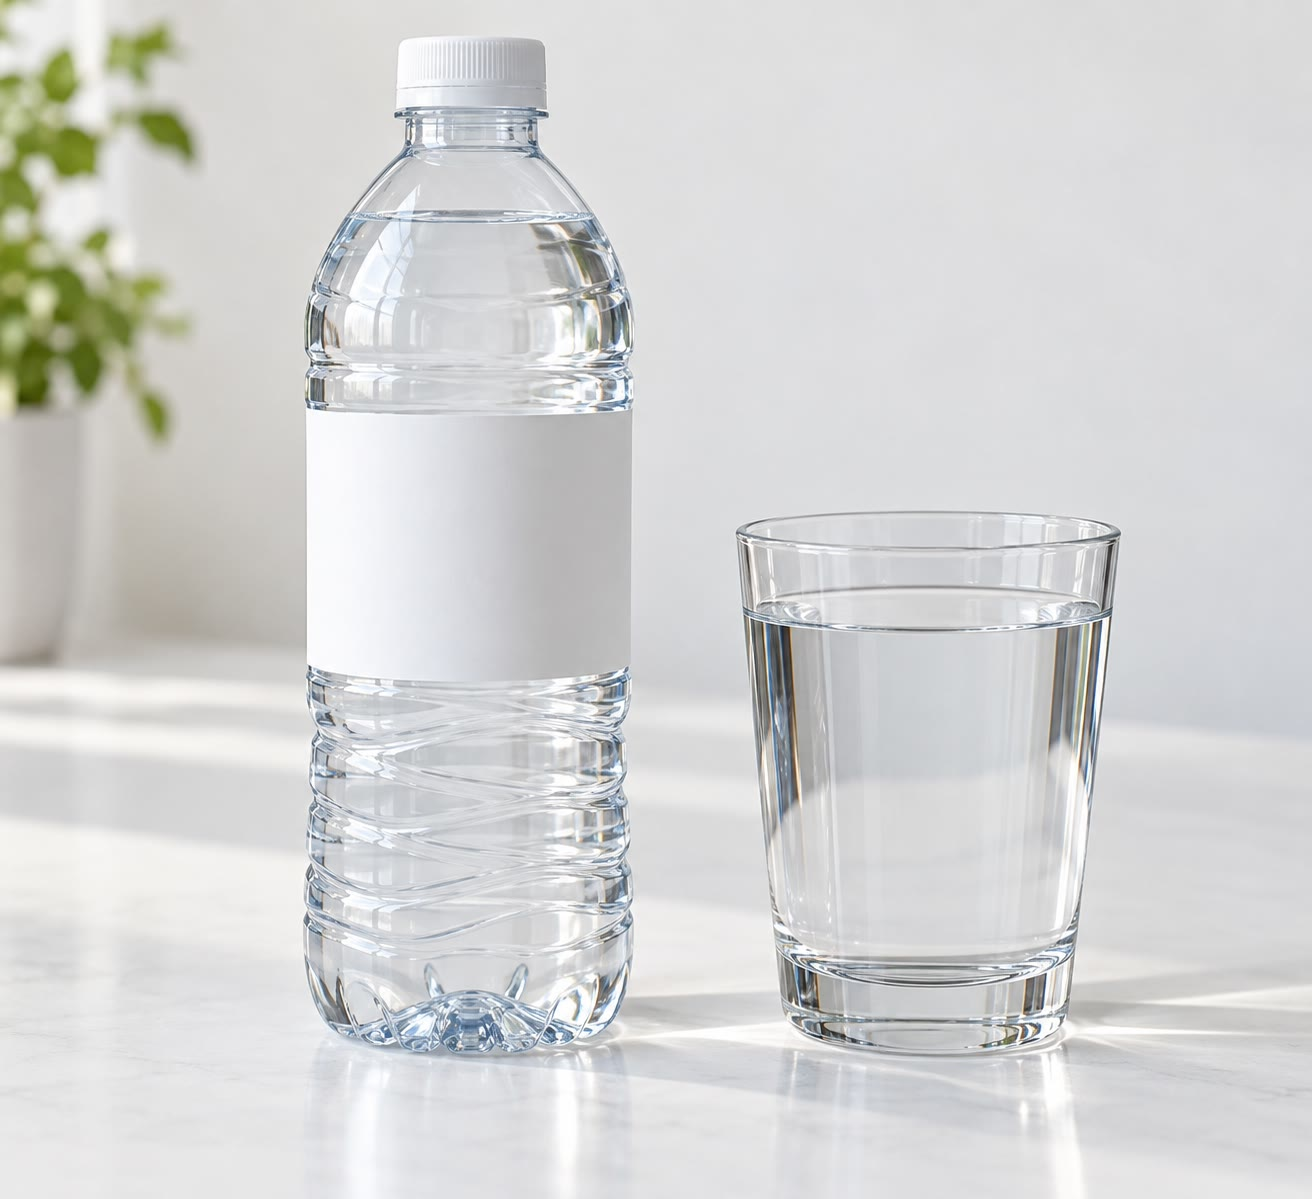
\includegraphics[width=0.5\linewidth]{images/book1/ai/g6-mineral-water.jpg}

{\small Uma garrafa de água mineral: límpida e incolor, e mesmo assim
uma \omterm{def:g6:pure-substances-and-mixtures:mixture}{mistura}.}
\end{omfigure}

\begin{example}[Ler o rótulo de uma água mineral]\label{ex:g6:pure-substances-and-mixtures:label}
Um rótulo diz: cálcio \qty{78}{mg/L}, magnésio \qty{24}{mg/L}, sódio
\qty{5}{mg/L}, hidrogenocarbonato (bicarbonato) \qty{357}{mg/L},
sulfato \qty{10}{mg/L}, cloreto \qty{4}{mg/L}. (Esses números são um
exemplo.) Em um litro há $78 + 24 + 5 + 357 + 10 + 4 = 478$\,mg de
substâncias dissolvidas, cerca de meio grama: muito pouco ao lado dos
\qty{1000}{g} de água, mas o bastante para fazer dela uma \omterm{def:g6:pure-substances-and-mixtures:mixture}{mistura}.
\end{example}

\section{Exercícios}

\begin{exercise}[$\star$]\label{exo:g6:pure-substances-and-mixtures:1}
\omterm{def:g6:pure-substances-and-mixtures:pure-substance}{Substância pura} ou \omterm{def:g6:pure-substances-and-mixtures:mixture}{mistura}? Água destilada, \omterm{def:g4:air-a-mixture-of-gases:air}{ar}, água do mar, um bloco
de ferro puro, leite, um cristal de açúcar.
\end{exercise}

\begin{exercise}[$\star$]\label{exo:g6:pure-substances-and-mixtures:2}
Homogênea ou heterogênea? Água salgada, granito, óleo sobre água, água da
torneira, granola.
\end{exercise}

\begin{exercise}[$\star$]\label{exo:g6:pure-substances-and-mixtures:3}
O que é uma \omterm{def:g6:pure-substances-and-mixtures:species}{espécie química}? Dê três exemplos.
\end{exercise}

\begin{exercise}[$\star$]\label{exo:g6:pure-substances-and-mixtures:4}
Um líquido ferve a \qty{78}{\celsius}, e a temperatura dele fica em
\qty{78}{\celsius} enquanto ele ferve. Use a tabela de constantes para
sugerir o que ele é.
\end{exercise}

\begin{exercise}[$\star$]\label{exo:g6:pure-substances-and-mixtures:5}
Por que o ``suco de laranja puro'' não é uma \omterm{def:g6:pure-substances-and-mixtures:pure-substance}{substância pura} para um
químico?
\end{exercise}

\begin{exercise}[$\star\star$]\label{exo:g6:pure-substances-and-mixtures:6}
Um líquido começa a ferver a \qty{100.5}{\celsius} e a temperatura dele
sobe enquanto ele ferve. Ele é uma \omterm{def:g6:pure-substances-and-mixtures:pure-substance}{substância pura}? O que ele poderia
ser?
\end{exercise}

\begin{exercise}[$\star\star$]\label{exo:g6:pure-substances-and-mixtures:7}
Olhe a figura dos quatro béqueres. Em que béquer um filtro poderia
separar as partes da \omterm{def:g6:pure-substances-and-mixtures:mixture}{mistura}? Em qual não poderia?
\end{exercise}

\begin{exercise}[$\star\star$]\label{exo:g6:pure-substances-and-mixtures:8}
Um cubo de metal de volume \qty{10}{cm^3} tem massa \qty{78.7}{g}. Qual
é a massa de \qty{1}{cm^3}? Que metal da tabela ele poderia ser?
\end{exercise}

\begin{exercise}[$\star\star$]\label{exo:g6:pure-substances-and-mixtures:9}
Com o rótulo de água mineral do exemplo, que porcentagem da massa
dissolvida é hidrogenocarbonato? Arredonde para o número inteiro mais
próximo.
\end{exercise}

\begin{exercise}[$\star\star$]\label{exo:g6:pure-substances-and-mixtures:10}
A água do mar contém cerca de \qty{35}{g} de sais por quilograma. Que
massa de sais há num balde de \qty{2}{kg} de água do mar? Que
porcentagem da massa da água do mar é sal?
\end{exercise}

\begin{exercise}[$\star\star\star$]\label{exo:g6:pure-substances-and-mixtures:11}
Dois líquidos límpidos e incolores parecem idênticos. Descreva duas
medidas, feitas num laboratório, que mostrariam se eles são a mesma
\omterm{def:g6:pure-substances-and-mixtures:pure-substance}{substância pura}.
\end{exercise}

\begin{exercise}[$\star\star\star$]\label{exo:g6:pure-substances-and-mixtures:12}
Uma \omterm{def:g6:pure-substances-and-mixtures:mixture}{mistura} é feita de \qty{90}{g} de água e \qty{10}{g} de etanol. Que
porcentagem da massa dela é etanol? Ela pode ser identificada com a
tabela de constantes? Explique.
\end{exercise}

\section{Problema: três líquidos incolores}

\begin{problem}[{Problema de fim de semana --- três frascos sem rótulo
de um líquido límpido e incolor, e as medidas que os distinguem}]
\label{pb:g6:pure-substances-and-mixtures:1}
% ledger: bp:water, bp:ethanol, rho:water, rho:ethanol, rho:seawater, sea:salinity
Um técnico de laboratório encontra três frascos, A, B e C, cujos rótulos
caíram. Os três contêm um líquido límpido e incolor. O laboratório só
usa três líquidos desse tipo: água destilada, etanol e água do mar
trazida de uma saída de campo. O técnico faz três tipos de medidas, no
laboratório.

\medskip
\noindent\textbf{Parte I --- Olhar.}
\begin{enumerate}
  \item Os três líquidos parecem exatamente iguais. O técnico consegue
        saber, olhando, quais deles são \omterm{def:g6:pure-substances-and-mixtures:pure-substance}{substâncias puras}? Explique.
  \item Se um deles for uma \omterm{def:g6:pure-substances-and-mixtures:mixture}{mistura}, ela é homogênea ou heterogênea?
  \item Que tipo de medida pode mostrar que um líquido é uma \omterm{def:g6:pure-substances-and-mixtures:pure-substance}{substância
        pura}?
\end{enumerate}

\medskip
\noindent\textbf{Parte II --- Medir.}
Cada líquido é aquecido até ferver. O líquido A ferve a
\qty{100}{\celsius} e a temperatura dele fica nesse valor. O líquido B
ferve a \qty{78}{\celsius} e fica nesse valor. O líquido C começa a
ferver a \qty{100.6}{\celsius}, e a temperatura dele continua subindo
devagar. Depois, \qty{50.0}{mL} de cada líquido são pesados: A
\qty{49.8}{g}, B \qty{39.5}{g}, C \qty{51.2}{g}.
\begin{enumerate}[resume]
  \item Que líquidos são \omterm{def:g6:pure-substances-and-mixtures:pure-substance}{substâncias puras}? Qual é uma \omterm{def:g6:pure-substances-and-mixtures:mixture}{mistura}?
  \item Com a tabela de constantes deste capítulo, dê o nome dos
        líquidos A e B.
  \item Calcule a massa de \qty{1}{mL} (isto é, \qty{1}{cm^3}) de cada
        líquido.
  \item Essas massas concordam com a sua resposta à questão 5?
  \item Por que a temperatura do líquido C continua subindo enquanto ele
        ferve?
\end{enumerate}

\medskip
\noindent\textbf{Parte III --- O que há no líquido C?}
Deixam-se \qty{100}{mL} do líquido C secar num recipiente. Quando toda a
água foi embora, restam \qty{3.5}{g} de cristais brancos.
\begin{enumerate}[resume]
  \item O que esse resíduo mostra sobre o líquido C?
  \item Com a massa de \qty{1}{mL} de C encontrada na questão 6, calcule
        a massa de \qty{100}{mL} de C e depois a porcentagem da massa
        dele que é sal (com uma casa decimal).
  \item A água do mar contém cerca de \qty{35}{g} de sais em cada
        quilograma. Que porcentagem é essa? Compare com a questão 10.
  \item Conclua: quantos gramas de sal cada litro do líquido C contém, e
        o líquido C é a água do mar?
\end{enumerate}
\end{problem}